% section43.tex

%%%%%% Section %%%%%%

\section{\caseENGRUS{Natural transformations}{ / }{Естественные преобразования}}\label{sec:nat trans}

In this section we conclude our discussion of the {\bf Big 3}, by defining natural transformations. Category theory was originally invented to discuss natural transformations. These were sufficiently conceptually challenging that they required formalization and thus the invention of category theory. If we think of categories as domains (of discourse, interaction, comparability, etc.) and of functors as transformations between different domains, the natural transformations compare different transformations.

Natural transformations can seem a bit abstruse at first, but hopefully some examples and exercises will help.

%%%% Subsection %%%%

\subsection{\caseENGRUS{Definition and examples}{ / }{Определение и примеры}}

Let's begin with an example. There is a functor $\List\taking\Set\to\Set$, which sends a set $X$ to the set $\List(X)$ consisting of all lists whose entries are elements of $X$. Given a morphism $f\taking X\to Y$, we can transform a list with entries in $X$ into a list with entries in $Y$ by applying $f$ to each (this was worked out in Exercise \ref{exc:list as functor}).\index{a functor!$\List\taking\Set\to\Set$}. 

It may seem a strange thing to contemplate, but there is also a functor $\List\circ\List\taking\Set\to\Set$ that sends a set $X$ to the set of lists of lists in $X$. If $X=\{a,b,c\}$ then $\List\circ\List(X)$ contains elements like $\big[[a,b],[a,c,a,b,c],[c]\big]$ and $\big[[\;]\big]$ and $\big[[a],[\;],[a,a,a]\big]$. We can {\em naturally transform} a list of lists into a list by concatenation. In other words, for any set $X$ there is a function $\mu_X\taking\List\circ\List(X)\to\List(X)$ which sends our lists above to $[a,b,a,c,a,b,c,c]$ and $[\;]$ and $[a,a,a,a]$, respectively. In fact, even if we use a function $f\taking X\to Y$ to convert a list of $X$'s into a list of $Y$'s (or a list of lists of $X$'s into a list of lists of $Y$'s), the concatenation “works right”. Take a deep breath for the precise statement couched as a slogan.

\begin{slogan}
Naturality works like this: Using a function $f\taking X\to Y$ to convert a list of lists of $X$'s into a list of list of $Y$'s and then concatenating to get a simple list of $Y$'s {\bf does the same thing as} first concatenating our list of lists of $X$'s into a simple list of $X$'s and then using our function $f$ to convert it into a list of $Y$'s.
\end{slogan}

Let's make this concrete. Let $X=\{a,b,c\}$, let $Y=\{1,2,3\}$, and let $f\taking X\to Y$ assign $f(a)=1, f(b)=1, f(c)=2$. Our naturality condition says the following for any list of lists of $X$'s, in particular for $\big[[a,b],[a,c,a,b,c],[c]\big]$:
$$\xymatrix@=40pt{
\big[[a,b],[a,c,a,b,c],[c]\big]\ar@{|->}[r]^-{\mu_X}\ar@{|->}[d]_{\List\circ\List(f)}&[a,b,a,c,a,b,c,c]\ar@{|->}[d]^{\List(f)}\\
\big[[1,1],[1,2,1,1,2],[2]\big]\ar@{|->}[r]_-{\mu_Y}&[1,1,1,2,1,1,2,2]
}
$$

Keep these $\mu_X$ in mind in the following definition—they serve as the “components” of a natural transformation $\List\circ\List\to\List$ of functors $\mcC\to\mcD$, where $\mcC=\mcD=\Set$.

\begin{definition}\label{def:natural transformation}\index{natural transformation}

Let $\mcC$ and $\mcD$ be categories and let $F\taking\mcC\to\mcD$ and $G\taking\mcC\to\mcD$ be functors. A {\em natural transformation $\alpha$ from $F$ to $G$}, denoted $\alpha\taking F\to G$, is defined as follows: one announces some constituents (A. components) and asserts that they conform to some laws (1. naturality squares). Specifically, one announces
\begin{enumerate}[\hsp A.]
\item for each object $c\in\Ob(\mcC)$ a morphism $\alpha_c\taking F(c)\to G(c)$ in $\mcD$, called {\em the $c$-component of $\alpha$}.\index{component}
\end{enumerate}
One asserts that the following law holds:
\begin{enumerate}[\hsp 1.]
\item For every morphism $h\taking c\to c'$ in $\mcC$, the following square, called the {\em naturality square for $h$}, must commute:
\begin{align}\label{dia:naturality square}
\xymatrix{F(c)\ar@{}[dr]|{\checkmark}\ar[d]_{F(h)}\ar[r]^{\alpha_c}&G(c)\ar[d]^{G(h)}\\F(c')\ar[r]_{\alpha_{c'}}&G(c')}
\end{align}
\end{enumerate}

\end{definition}

\begin{example}

Consider the categories $\mcC\iso[1]$ and $\mcD\iso[2]$ drawn below:
$$\mcC:=\fbox{\xymatrix{\LMO{0}\ar[r]^p&\LMO{1}
}}
\hspace{.5in}
\mcD:=\fbox{\xymatrix{\LMO{A}\ar[r]^f&\LMO{B}\ar[r]^g&\LMO{C}.
}}
$$
Consider the functors $F,G\taking[1]\to[2]$ where $F(0)=A$, $F(1)=B$, $G(0)=A$, and $G(1)=C$. The orange dots and arrows in the picture below represent the image of $\mcC$ under $F$ and $G$.

\begin{center}
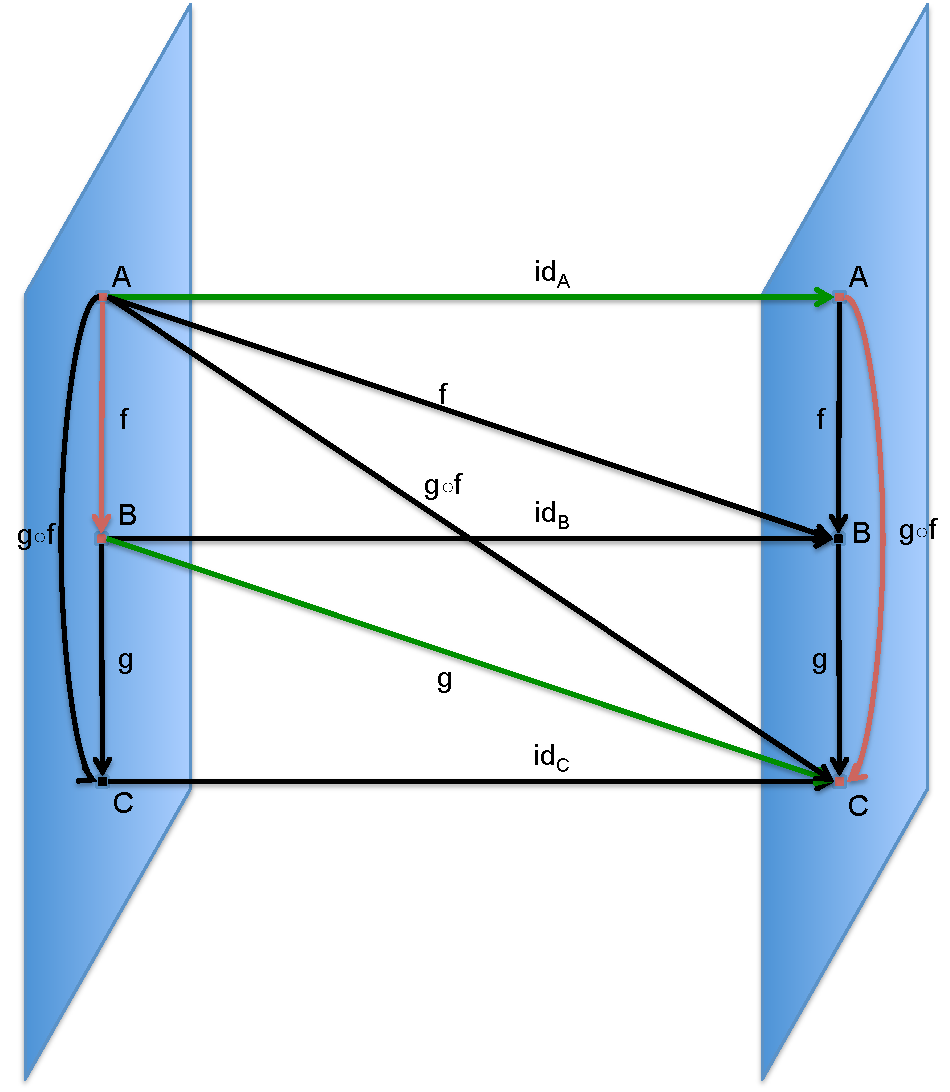
\includegraphics[height=4in]{natTrans}
\end{center}

It turns out that there is only one possible natural transformation $F\to G$; we call it $\alpha$ and explore its naturality square. We have drawn the components of $\alpha\taking F\to G$ in green. These components are $\alpha_0=\id_A\taking F(0)\to G(0)$ and $\alpha_1=g\taking F(1)\to G(1)$. The naturality square for $p\taking 0\to 1$ is written twice below, once with notation following that in (\ref{dia:naturality square}) and once in local notation.
$$
\xymatrix{
F(0)\ar[r]^{\alpha_0}\ar[d]_{F(p)}&G(0)\ar[d]^{G(p)}\\
F(1)\ar[r]_{\alpha_1}&G(1)}
\hspace{.6in}
\xymatrix{
A\ar[r]^{\id_A}\ar[d]_{f}&A\ar[d]^{g\circ f}\\
B\ar[r]_{g}&C
}
$$
It is clear that this diagram commutes, so our components $\alpha_0$ and $\alpha_1$ satisfy the law of Definition \ref{def:natural transformation}, making $\alpha$ a natural transformation.

\end{example}

\begin{lemma}\label{lemma:generators for nattrans}

Let $\mcC$ and $\mcD$ be categories, let $F,G\taking\mcC\to\mcD$ be functors, and for every object $c\in\Ob(\mcC)$, let $\alpha_c\taking F(c)\to G(c)$ be a morphism in $\mcD$. Suppose given a path $c_0\To{f_1}c_1\To{f_2}\cdots\To{f_n} c_n$ such that the naturality square 
$$
\xymatrix{F(c_{i-1})\ar[d]_{F(f_i)}\ar[r]^{\alpha_{c_{i-1}}}&G(c_{i-1})\ar[d]^{G(f_i)}\\F(c_i)\ar[r]_{\alpha_{c_i}}&G(c_i)
}
$$
commutes for each $1\leq i\leq n$. Then the naturality square for the composite $p:=f_n\circ\cdots\circ f_2\circ f_1\taking c_0\to c_n$ 
$$\xymatrix{F(c_0)\ar[r]^{\alpha_{c_0}}\ar[d]_{F(p)}&G(c_0)\ar[d]^{G(p)}\\F(c_n)\ar[r]_{\alpha_{c_n}}&G(c_n)}
$$
also commutes. In particular, the naturality square commutes for every identity morphism $\id_c$.

\end{lemma}

\begin{proof}

When $n=0$ we have a path of length 0 starting at each $c\in\Ob(\mcC)$. It vacuously satisfies the condition, so we need to see that its naturality square 
$$\xymatrix{F(c)\ar[r]^{\alpha_c}\ar[d]_{F(\id_c)}&G(c)\ar[d]^{G(\id_c)}\\F(c)\ar[r]_{\alpha_c}&G(c)}
$$
commutes. But this is clear because functors preserve identities. 

The rest of the proof follows by induction on $n$. Suppose $q=f_{n-1}\circ\cdots\circ f_2\circ f_1\taking c_0\to c_{n-1}$ and $p=f_n\circ q$ and that the naturality squares for $q$ and for $f_n$ commute; we need only show that the naturality square for $p$ commutes. That is, we assume the two small squares commute below; but it follows that the large rectangle does too, completing the proof.

$$
\xymatrix{
F(c_0)\ar[r]^{\alpha_{c_0}}\ar[d]_{F(q)}&G(c_0)\ar[d]^{G(q)}\\
F(c_{n-1})\ar[r]^{\alpha_{c_{n-1}}}\ar[d]_{F(f_n)}&G(c_{n-1})\ar[d]^{G(f_n)}\\
F(c_n)\ar[r]^{\alpha_{c_n}}&G(c_n)
}
$$

\end{proof}

\begin{example}\label{ex:nattrans [1]}

Let $\color{red}{\mcC}=\color{blue}{\mcD}=\color{black}{[1]}$ be the linear order of length 1, thought of as a category (by Proposition \ref{prop:preorders to cats}). There are three functors $\mcC\to\mcD$, which we can write as $(0,0), (0,1),$ and $(1,1)$; these are depicted left to right below.
$$\xymatrix{
\LMO{\color{red}{0}}\ar@{|->}[r]\ar@[red][d]_f&\LMO{\color{blue}{0}}\ar@[blue][d]^f&&\LMO{\color{red}{0}}\ar@{|->}[r]\ar@[red][d]_f&\LMO{\color{blue}{0}}\ar@[blue][d]^f&&\LMO{\color{red}{0}}\ar@{|->}[dr]\ar@[red][d]_f&\LMO{\color{blue}{0}}\ar@[blue][d]^f\\
\LMO{\color{red}{1}}\ar@{|->}[ur]&\LMO{\color{blue}{1}}&&\LMO{\color{red}{1}}\ar@{|->}[r]&\LMO{\color{blue}{1}}&&\LMO{\color{red}{1}}\ar@{|->}[r]&\LMO{\color{blue}{1}}
}
$$
These are just functors so far. What are the natural transformations say $\alpha\taking (0,0)\to(0,1)$? To specify a natural transformation, we must specify a component for each object in $\mcC$. In our case $\alpha_0\taking 0\to 0$ and $\alpha_1\taking 0\to 1$. There is only one possible choice: $\alpha_0=\id_0$ and $\alpha_1=f$. Now that we have chosen components we need to check the naturality squares. 

There are three morphisms in $\mcC$, namely $\id_0, f, \id_1$. By Lemma \ref{lemma:generators for nattrans}, we need only check the naturality square for $f$. We write it twice below, once in the abstract notation and once in concrete notation:
$$
\xymatrix{
F(0)\ar[r]^{\alpha_0}\ar[d]_{F(f)}&G(0)\ar[d]^{G(f)}\\
F(1)\ar[r]_{\alpha_1}&G(1)
}\hspace{.5in}
\xymatrix{
0\ar[r]^{\id_0}\ar[d]_{\id_0}&0\ar[d]^{f}\\
0\ar[r]_{f}&1
}
$$
This commutes, so $\alpha$ is indeed a natural transformation.

\end{example}

\begin{exercise}
With notation as in Example \ref{ex:nattrans [1]},
\sexc how many natural transformations are there $(0,0)\to (1,1)$?
\item how many natural transformations are there $(0,0)\to (0,0)$?
\item how many natural transformations are there $(0,1)\to (0,0)$?
\item how many natural transformations are there $(0,1)\to (1,1)$?
\endsexc
\end{exercise}

\begin{exercise}
Let $\List\taking\Set\to\Set$ be the functor sending a set $X$ to the set $\List(X)$ of lists with entries in $X$. We saw above that there is a natural transformation $\List\circ\List\to\List$ given by concatenation.
\sexc If someone said “singleton lists give a natural transformation $\sigma$ from $\id_\Set$ to $\List$”, what might they mean? That is, for a set $X$, what component $\sigma_X$ might they be suggesting?
\item Do these components satisfy the necessary naturality squares for functions $f\taking X\to Y$?
\endsexc
\end{exercise}

\begin{exercise}
Let $\mcC$ and $\mcD$ be categories, and suppose that $d\in\Ob(\mcD)$ is a terminal object. Consider the functor $\{d\}^\mcC\taking\mcC\to\mcD$ that sends each object $c\in\Ob(\mcC)$ to $d$ and each morphism in $\mcC$ to the identity morphism $\id_d$ on $d$. 
\sexc For any other functor $F\taking\mcC\to\mcD$, how many natural transformations are there $F\to\{d\}^\mcC$? 
\item Let $\mcD=\Set$ and let $d=\singleton$. If $\mcC=[1]$ is the linear order of length 1, and $F\taking\mcC\to\Set$ is any functor, what does it mean to give a natural transformation $\{d\}^\mcC\to F$?
\endsexc
\end{exercise}

\begin{application}\label{app:change of fsm}\index{natural transformation!as refinement of model}

In Figure \ref{fig:fsa} we drew a \href{http://en.wikipedia.org/wiki/Finite-state_machine}{finite state machine} on alphabet $\Sigma=\{a,b\}$, and in Example \ref{ex:action table} we showed the associated action table. It will be reproduced below. Imagine this was your model for understanding the behavior of some system when acted on by commands $a$ and $b$. And suppose that a collaborator tells you that she has a more refined notion that fits with the same data. Her notion has 6 states rather than 3, but it's “compatible”. What might that mean? 

Let's call the original state machine $X$ and the new model $Y$.

\begin{center}
\parbox{1.9in}{\boxtitle{$X$:=}\fbox{
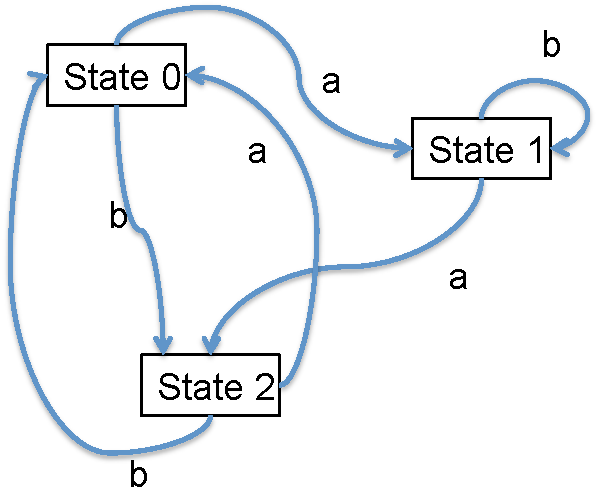
\includegraphics[height=1.5in]{FSM1}
}}
\hsp
\parbox{2.6in}{\boxtitle{$Y$:=}\fbox{
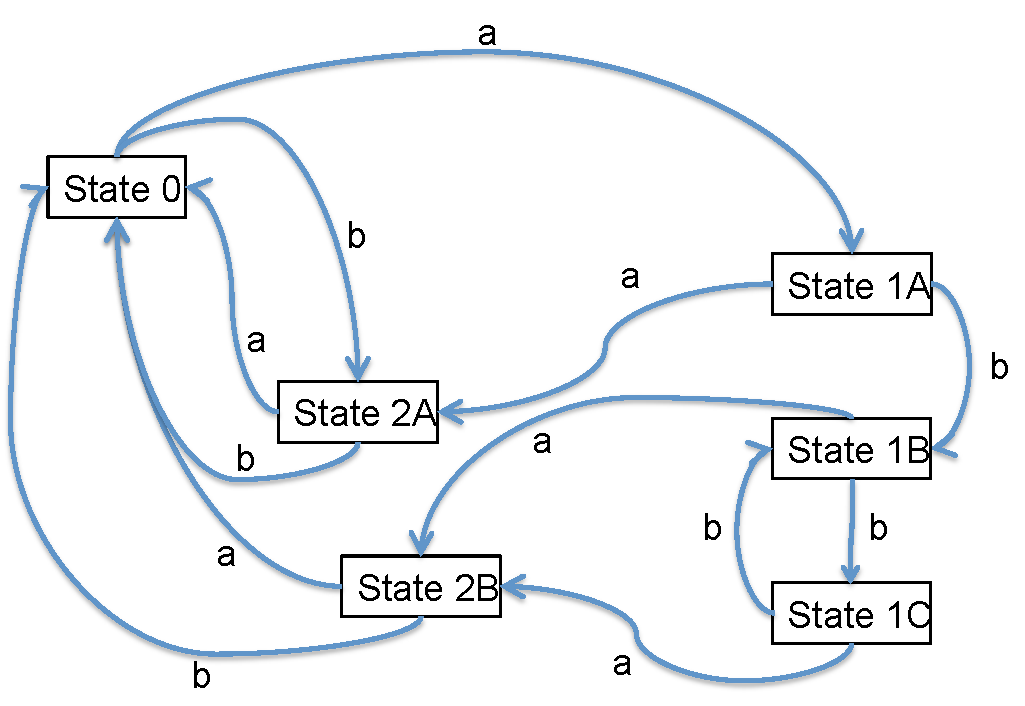
\includegraphics[height=1.7in]{FSM2}
}}
\end{center}

The action tables for these two machines are:
\begin{center}
\begin{tabular}{| l || l | l |}\bhline
\multicolumn{3}{|c|}{Original model $X$}\\\bhline
{\bf ID}&{\bf a}&{\bf b}\\\bbhline
State 0&State 1&State 2\\\hline
State 1& State 2& State 1\\\hline
State 2&State 0&State 0\\\bhline
\end{tabular}
\hspace{.5in}
\begin{tabular}{| l || l | l |}\bhline
\multicolumn{3}{|c|}{Proposed model $Y$}\\\bhline
{\bf ID}&{\bf a}&{\bf b}\\\bbhline
State 0&State 1A&State 2A\\\hline
State 1A& State 2A& State 1B\\\hline
State 1B& State 2B& State 1C\\\hline
State 1C&State 2B&State 1B\\\hline
State 2A&State 0&State 0\\\hline
State 2B&State 0&State 0\\\bhline
\end{tabular}
\end{center}

How are these models compatible? Looking at the table for $Y$, if one removes the distinction between States 1A, 1B, 1C and between States 2A and 2B, then one returns with the table for $X$. The table for $Y$ is more specific, but it is fully compatible with table $X$. The sense in which it is compatible is precisely the sense defined by there being a natural transformation.

Recall that $\mcM=(\List(\Sigma),[\;],\plpl)$ is a monoid, and that a monoid is simply a category with one object, say $\Ob(\mcM)=\{\monOb\}$ (see Section \ref{sec:mon grp pro as cat}). With $\Sigma=\{a,b\}$, the monoid $\mcM$ can be visualized as follows:
$$
\mcM=\fbox{\xymatrix{\LMO{\monOb}\ar@(ul,dl)[]_a\ar@(ur,dr)[]^b}}
$$
Recall also that a state machine on $\mcM$ is simply a functor $\mcM\to\Set$. We thus have two such functors, $X$ and $Y$. A natural transformation $\alpha\taking Y\to X$ would consist of a component $\alpha_m$ for every object $m\in\Ob(\mcM)$, such that certain diagrams commute. But $\mcM$ having only one object, we need only one function $\alpha_\monOb\taking Y(\monOb)\to X(\monOb)$, where $Y(\monOb)$ is the set of (6) states of $Y$ and $X(\monOb)$ is the set of (3) states of $X$.

The states of $Y$ have been named so as to make the function $\alpha_\monOb$ particularly easy to guess.\footnote{The function $\alpha_\monOb\taking Y(\monOb)\to X(\monOb)$ makes the following assignments: $\tn{State 0}\mapsto \tn{State 0}, \tn{State 1A}\mapsto \tn{State 1}, \tn{State 1B}\mapsto \tn{State 1}, \tn{State 1C}\mapsto \tn{State 1}, \tn{State 2A}\mapsto \tn{State 2}, \tn{State 2B}\mapsto \tn{State 2}.$} We need to check that two squares commute:
\begin{align}\label{dia:naturality squares for fsm}
\xymatrix{Y(\monOb)\ar[r]^{\alpha_\monOb}\ar[d]_{Y(a)}&X(\monOb)\ar[d]^{X(a)}\\Y(\monOb)\ar[r]_{\alpha_\monOb}&X(\monOb)
}
\hspace{.5in}
\xymatrix{Y(\monOb)\ar[r]^{\alpha_\monOb}\ar[d]_{Y(b)}&X(\monOb)\ar[d]^{X(b)}\\Y(\monOb)\ar[r]_{\alpha_\monOb}&X(\monOb)
}
\end{align}
This can only be checked by going through and making sure certain things match, as specified by (\ref{dia:naturality squares for fsm}); we spell it out in gory detail. The columns that should match are those whose entries are written in blue.

\begin{align}\label{dia:naturality for a}
\begin{tabular}{| l || l | l | l | l |}
\bhline
\multicolumn{5}{|c|}{Naturality square for $a\taking \monOb\to\monOb$}\\\bhline
{\bf $Y(\monOb)$\; [ID]}&{\bf $Y(a)$}&{\bf $\alpha_\monOb\circ Y(a)$}&{\bf $\alpha_\monOb$}&{\bf $X(a)\circ\alpha_\monOb$}\\\bbhline
State 0&State 1A&\color{blue}{State 1}&State 0&\color{blue}{State 1}\\\hline
State 1A& State 2A&\color{blue}{State 2}&State 1&\color{blue}{State 2}\\\hline
State 1B& State 2B&\color{blue}{State 2}&State 1&\color{blue}{State 2}\\\hline
State 1C&State 2B&\color{blue}{State 2}&State 1&\color{blue}{State 2}\\\hline
State 2A&State 0&\color{blue}{State 0}&State 2&\color{blue}{State 0}\\\hline
State 2B&State 0&\color{blue}{State 0}&State 2&\color{blue}{State 0}\\\bhline
\end{tabular}
\end{align}
\begin{align}\label{dia:naturality for b}
\begin{tabular}{| l || l | l | l | l |}
\bhline
\multicolumn{5}{|c|}{Naturality square for $b\taking\monOb\to\monOb$}\\\bhline
{\bf $Y(\monOb)$\; [ID]}&{\bf $Y(b)$}&{\bf $\alpha_\monOb\circ Y(b)$}&{\bf $\alpha_\monOb$}&{\bf $X(b)\circ\alpha_\monOb$}\\\bbhline
State 0&State 2A&\color{blue}{State 2}&State 0&\color{blue}{State 2}\\\hline
State 1A& State 1B&\color{blue}{State 1}&State 1&\color{blue}{State 1}\\\hline
State 1B& State 1C&\color{blue}{State 1}&State 1&\color{blue}{State 1}\\\hline
State 1C&State 1B&\color{blue}{State 1}&State 1&\color{blue}{State 1}\\\hline
State 2A&State 0&\color{blue}{State 0}&State 2&\color{blue}{State 0}\\\hline
State 2B&State 0&\color{blue}{State 0}&State 2&\color{blue}{State 0}\\\bhline
\end{tabular}
\end{align}

In reality we need to check that for {\em every} morphism in $\mcM$, such as $[a,a,b]$, a similar diagram commutes. But this holds automatically. For example (flipping the naturality square sideways for typographical reasons)
$$
\xymatrix{
Y(\monOb)\ar[r]^{Y(a)}\ar[d]^{\alpha_\monOb}&Y(\monOb)\ar[r]^{Y(a)}\ar[d]^{\alpha_\monOb}&Y(\monOb)\ar[r]^{Y(b)}\ar[d]^{\alpha_\monOb}&Y(\monOb)\ar[d]^{\alpha_\monOb}\\
X(\monOb)\ar[r]_{X(a)}&X(\monOb)\ar[r]_{X(a)}&X(\monOb)\ar[r]_{X(b)}&X(\monOb)
}
$$
Since each small square above commutes (as checked by tables \ref{dia:naturality for a} and \ref{dia:naturality for b}), the big outer rectangle commutes too.

To recap, the notion of compatibility between $Y$ and $X$ is one that can be checked and agreed upon by humans, but doing so it is left implicit, and it may be difficult to explain to an outsider what exactly was agreed to, especially in more complex situations. It is quite convenient to simply claim “there is a natural transformation from $Y$ to $X$.”

\end{application}

\begin{exercise}\label{exc:id nat trans}
Let $F\taking\mcC\to\mcD$ be a functor. Suppose someone said “the identity on $F$ is a natural transformation from $F$ to itself.” \sexc What might they mean?
\item If it is somehow true, what are the components of this natural transformation?
\endsexc
\end{exercise}

\begin{example}

Let $[1]\in\Ob(\Cat)$ be the free arrow category described in Exercise \ref{exc:[1]} and let $\mcD$ be any category. To specify a functor $F\taking[1]\to\mcD$ requires the specification of two objects, $F(v_1), F(v_2)\in\Ob(\mcD)$ and a morphism $F(e)\taking F(v_1)\to F(v_2)$ in $\mcD$. The identity and composition formulas are taken care of once that much is specified. To recap, a functor $F\taking[1]\to\mcD$ is the same thing as a morphism in $\mcD$.

Thus, choosing two functors $F,G\taking[1]\to\mcD$ is precisely the same thing as choosing two morphisms in $\mcD$. Let us call them $f\taking a_0\to a_1$ and $g\taking b_0\to b_1$, where to be clear we have $f=F(e), a_0=F(v_0), a_1=F(v_1)$ and $g=G(e), b_0=G(v_0), b_1=G(v_1)$. 

A natural transformation $\alpha\taking F\to G$ consists of two components, $h_0:=\alpha_{v_0}\taking a_0\to b_0$ and $h_1:=\alpha_{v_1}\taking a_1\to b_1$, drawn as dashed lines below:
$$\xymatrix{a_0\ar@{-->}[r]^{h_0}\ar[d]_f&b_0\ar[d]^{g}\\a_1\ar@{-->}[r]_{h_1}&b_1}$$
The condition for $\alpha$ to be a natural transformation is that the above square commutes. 

In other words, a functor $[1]\to\mcD$ is an arrow in $\mcD$ and a natural transformation between two such functors is just a commutative square in $\mcD$.

\end{example}

\begin{example}\label{ex:graph to paths}

Recall that to any graph $G$ we can associate the so-called paths-graph $\Paths(G)$, as described in Example \ref{ex:paths-graph}. This is a functor $\Paths\taking\Grph\to\Grph$.\index{a functor!$\Paths\taking\Grph\to\Grph$} There is also an identity functor $\id_{\Grph}\taking\Grph\to\Grph$. A natural transformation $\eta\taking\id_\Grph\to\Paths$ would consist of a graph homomorphism $\eta_G\taking \id_\Grph(G)\to\Paths(G)$ for every graph $G$. But $\id_\Grph(G)=G$ by definition, so we need $\eta_G\taking G\to\Paths(G)$. Recall that $\Paths(G)$ has the same vertices as $G$ and every arrow in $G$ counts as a path (of length 1). So there is an obvious graph homomorphism from $G$ to $\Paths(G)$. It is not hard to see that the necessary naturality squares commute.

\end{example}

\begin{example}\label{ex:concat paths of paths}

For any graph $G$ we can associate the paths-graph $\Paths(G)$, and nothing stops us from doing that twice to yield a new graph $\Paths(\Paths(G))$. Let's think through what a path of paths in $G$ is. It's a head-to-tail sequence of arrows in $\Paths(G)$, meaning a head-to-tail sequence of paths in $G$. These composable sequences of paths (or “paths of paths”) are the individual arrows in $\Paths(\Paths(G))$. (The vertices in $\Paths(G)$ and $\Paths(\Paths(G))$ are the same as those in $G$, and all source and target functions are as expected.)

Clearly, given such a sequence of paths in $G$, we could compose them to one big path in $G$ with the same endpoints. In other words, there is graph morphism $\mu_G\taking\Paths(\Paths(G))\to\Paths(G)$, that one might call “concatenation”. In fact, this concatenation extends to a natural transformation $$\mu\taking\Paths\circ\Paths\to\Paths$$ between functors $\Grph\to\Grph$. In Example \ref{ex:graph to paths}, we compared a graph to its paths-graph using a natural transformation $\id_{\Grph}\to\Paths$; here we are making a similar kind of comparison.

\end{example}

\begin{remark}

In Example \ref{ex:graph to paths} we saw that there is a natural transformation sending each graph into its paths-graph. There is a formal sense in which a category is nothing more than a kind of reverse mapping. That is, to specify a category is the same thing as to specify a graph $G$ together with a graph homomorphism $\Paths(G)\to G$. The formalities involve monads, which we will discuss in Section \ref{sec:monads}.

\end{remark}

\begin{exercise}
Let $X$ and $Y$ be sets, and let $f\taking X\to Y$. There is a functor $C_X\taking\Grph\to\Set$ that sends every graph to the set $X$ and sends every morphism of graphs to the identity morphism $\id_X\taking X\to X$. This functor is called {\em the constant functor at $X$}. Similarly there is a constant functor $C_Y\taking\Grph\to\Set$.
\sexc Use $f$ to construct a natural transformation $C_X\to C_Y$.
\item What are its components?
\endsexc
\end{exercise}

\begin{exercise}
For any graph $(V,A,src,tgt)$ we can extract the set of arrows or the set of vertices. Since each morphism of graphs includes a function between their arrow sets and a function between their vertex sets, we actually have functors $Ar\taking\Grph\to\Set$\index{a functor!$\Grph\to\Set$} and $V\!e\taking\Grph\to\Set$.
\sexc If someone said “taking source vertices gives a natural transformation from $Ar$ to $V\!e$”, what natural transfromation might they be referring to?
\item What are its components? 
\item If a different person, say from a totally different country, were to say “taking target vertices also gives a natural transformation from $Ar$ to $V\!e$,” would they also be correct?
\endsexc
\end{exercise}

\begin{example}[Graph homomorphisms are natural transformations]\label{ex:graph hom as NT}

As discussed above (see Diagram \ref{dia:graph index}), there is a category $\GrIn$ for which a functor $G\taking\GrIn\to\Set$ is the same thing as a graph. Namely, we have 
\begin{align*}
\GrIn:=\fbox{\GrInSchema}
\end{align*}
A natural transformation of two such functors $\alpha\taking G\to G'$ involves two components, $\alpha_{Ar}\taking G(Ar)\to G'(Ar)$ and $\alpha_{V\!e}\taking G(V\!e)\to G'(V\!e)$, and two naturality squares, one for $src$ and one for $tgt$. This is precisely the same thing as a graph homomorphism, as defined in Definition \ref{def:graph homomorphism}.

\end{example}

%%%% Subsection %%%%

\subsection{\caseENGRUS{Vertical and horizontal composition}{ / }{Вертикальная и горизонтальная композиция}}\label{sec:vert and hor}

In this section we discuss two types of compositions for natural transformations. The terms vertical and horizontal are used to describe them; these terms come from the following pictures:

$$
\parbox{1in}{\xymatrix{&\ar@{}[d]|(.65){\alpha\Down}\\\mcC\ar@/^2pc/[rr]^F\ar[rr]|G\ar@/_2pc/[rr]_H&&\mcD\\&\ar@{}[u]|(.65){\beta\Down}}}
\hspace{1in}
\parbox{2in}{\xymatrix{\mcC\ar@/^1.5pc/[rr]^{F_1}\ar@{}[rr]|{\gamma_1\Down}\ar@/_1.5pc/[rr]_{G_1}&&\mcD\ar@/^1.5pc/[rr]^{F_2}\ar@{}[rr]|{\gamma_2\Down}\ar@/_1.5pc/[rr]_{G_2}&&\mcE}}
$$
We generally use $\circ$ to denote both kinds of composition, but if we want to be very clear we will differentiate as follows: $\beta\circ\alpha\taking F\to H$ for vertical composition, and $\gamma_2\diamond\gamma_1\taking F_2\circ F_1\too G_2\circ G_1$ for horizontal composition. Of course, the actual arrangement of things on a page of text does not correlate with verticality or horizontality—these are just names. We will define them more carefully below.

%% Subsubsection %%

\subsubsection{\caseENGRUS{Vertical composition of natural transformations}{ / }{Вертикальная композиция естественных преобразований}}\index{natural transformation!vertical composition of}

The following proposition proves that functors and natural transformations (using vertical composition) form a category.

\begin{proposition}\label{prop:Fun(C,D)}

Let $\mcC$ and $\mcD$ be categories. There exists a category, called {\em the category of functors from $\mcC$ to $\mcD$} and denoted $\Fun(\mcC,\mcD)$\index{a symbol!$\Fun$}, whose objects are the functors $\mcC\to\mcD$ and whose morphisms are the natural transformations,
$$\Hom_{\Fun(\mcC,\mcD)}(F,G)=\{\alpha\taking F\to G\|\alpha\tn{ is a natural transformation}\}.$$That is, there are identity natural transformations, natural transformations can be composed, and the identity and associativity laws hold.

\end{proposition}

\begin{proof}

We showed in Exercise \ref{exc:id nat trans} that there for any functor $F\taking\mcC\to\mcD$, there is an identity natural transformation $\id_F\taking F\to F$ (its component at $c\in\Ob(\mcC)$ is $\id_{F(c)}\taking F(c)\to F(c)$). 

Given a natural transformation $\alpha\taking F\to G$ and a natural transformation $\beta\taking G\to H$, we propose for the composite $\beta\circ\alpha$ the transformation $\gamma\taking F\to H$ having components $\beta_c\circ\alpha_c$ for every $c\in\Ob(\mcC)$. To see that $\gamma$ is indeed a natural transformation, one simply puts together naturality squares for $\alpha$ and $\beta$ to get naturality squares for $\beta\circ\alpha$. 

The associativity and identity laws for $\Fun(\mcC,\mcD)$ follow from those holding for morphisms in $\mcD$.

\end{proof}

\begin{notation}
We sometimes denote the category $\Fun(\mcC,\mcD)$ by $\mcD^\mcC$. 
\end{notation}

\begin{example}

Recall from Exercise \ref{exc:Ob is a functor} that there is a functor $\Ob\taking\Cat\to\Set$\index{a functor!$\Ob\taking\Cat\to\Set$} sending a category to its set of objects. And recall from Example \ref{ex:discrete graph discrete cat} that there is a functor $Disc\taking\Set\to\Cat$\index{a functor!$Disc\taking\Set\to\Cat$} sending a set to the discrete category with that set of objects (all morphisms in $Disc(S)$ are identity morphisms). Let $P\taking\Cat\to\Cat$ be the composition $P=Disc\circ\Ob$. Then $P$ takes a category and makes a new category with the same objects but no morphisms. It's like crystal meth for categories.

Let $\id_\Cat\taking\Cat\to\Cat$ be the identity functor. There is a natural transformation $i\taking P\to\id_\Cat$. For any category $\mcC$, the component $i_\mcC\taking P(\mcC)\to\mcC$ is pretty easily understood. It is a morphism of categories, i.e. a functor. The two categories $P(\mcC)$ and $\mcC$ have the same set of objects, namely $\Ob(\mcC)$, so our functor is identity on objects; and $P(\mcC)$ has no non-identity morphisms, so nothing else needs be specified.

\end{example}

\begin{exercise}
Let $\mcC=\fbox{$\LMO{A}$}$ be the category with $\Ob(\mcC)=\{A\}$, and $\Hom_\mcC(A,A)=\{\id_A\}$. What is $\Fun(\mcC,\Set)$? In particular, characterize the objects and the morphisms.
\end{exercise}

\begin{exercise}
Let $n\in\NN$ and let $\ul{n}$ be the set with $n$ elements, considered as a discrete category.
\footnote{When we have a functor, such as $Disc\taking\Set\to\Cat$, we may sometimes say things like “Let $S$ be a set, considered as a category” (or in general, given a functor $F\taking\mcC\to\mcD$, we may say “consider $c\in\Ob(\mcC)$, taken as an object in $\mcD$”). What this means is that we want to take ideas and methods available in $\Cat$ and use them on our set $S$. Having our functor $Disc$ lying around, we use it to move $S$ into $\Cat$, as $Disc(S)\in\Ob(\Cat)$, upon which we can use our intended methods. However, our human minds get bogged down seeing $Disc(S)$ because it is bulky (e.g. $\Fun(Disc(\ul{3}),Disc(\ul{2}))$ is harder to read than $\Fun(\ul{3},\ul{2})$). So we abuse notation and write $S$ in place of  $Disc(S)$. To add insult to injury, we talk about $S$ as though it was still a set, e.g. discussing its elements rather than its objects. This kind of conceptual abbreviation is standard practice in mathematical discussion because it eases the mental burden for experts, but when one says “Let $S$ be an $X$ considered as a $Y$” the other may always ask, “How again are you considering $X$'s to be $Y$'s?” and expect a functor .}
In other words, we write $\ul{n}$ to mean what should really be called $Disc(\ul{n})$. Describe the category $\Fun(\ul{3},\ul{2})$.
\end{exercise}

\begin{exercise}
Let $\ul{1}$ denote the discrete category with one object, and let $\mcC$ be any category.
\sexc What are the objects of $\Fun(\ul{1},\mcC)$?
\item What are the morphisms of $\Fun(\ul{1},\mcC)$?
\endsexc
\end{exercise}

\begin{example}

Let $\ul{1}$ denote the discrete category with one object (also known as the trivial monoid). For any category $\mcC$, we investigate the category $\mcD:=\Fun(\mcC,\ul{1})$. Its objects are functors $\mcC\to\ul{1}$. Such a functor $F$ assigns to each object in $\mcC$ an object in $\ul{1}$ of which there is one; so there is no choice in what $F$ does on objects. And there is only one morphism in $\ul{1}$ so there is no choice in what $F$ does on morphisms. The upshot is that there is only one object in $\mcD$, let's call it $F$, in $\mcD$, so $\mcD$ is a monoid. What are its morphisms? 

A morphism $\alpha\taking F\to F$ in $\mcD$ is a natural transformation of functors. For every $c\in\Ob(\mcC)$ we need a component $\alpha_c\taking F(c)\to F(c)$, which is a morphism $1\to 1$ in $\ul{1}$. But there is only one morphism in $\ul{1}$, namely $\id_1$, so there is no choice about what these components should be: they are all $\id_1$. The necessary naturality squares commute, so $\alpha$ is indeed a natural transformation. Thus the monoid $\mcD$ is the trivial monoid; that is, $\Fun(\mcC,\ul{1})\iso\ul{1}$ for any category $\mcC$.

\end{example}

\begin{exercise}
Let $\ul{0}$ represent the discrete category on 0 objects; it has no objects and no morphisms. Let $\mcC$ be any category. What is $\Fun(\ul{0},\mcC)$?
\end{exercise}

\begin{exercise}
Let $[1]$ denote the free arrow category as in Exercise \ref{exc:[1]}, and let $\mcC$ be the graph indexing category from (\ref{dia:graph index}). Draw the underlying graph of the category $\Fun([1],\mcC)$, and then specify which pairs of paths in that graph correspond to commutative diagrams in $\Fun([1],\mcC)$.
\end{exercise}

%% Subsubsection %%

\subsubsection{\caseENGRUS{Natural isomorphisms}{ / }{Естественные изоморфизмы}}\index{natural isomorphism}

Let $\mcC$ and $\mcD$ be categories. We have defined a category $\Fun(\mcC,\mcD)$ whose objects are functors $\mcC\to\mcD$ and whose morphisms are natural transformations. What are the isomorphisms in this category? 

\begin{lemma}\label{lemma:natural iso}

Let $\mcC$ and $\mcD$ be categories and let $F,G\taking\mcC\to\mcD$ be functors. A natural transformation $\alpha\taking F\to G$ is an isomorphism in $\Fun(\mcC,\mcD)$ if and only if the component $\alpha_c\taking F(c)\to G(c)$ is an isomorphism for each object $c\in\Ob(\mcC)$. In this case $\alpha$ is called a {\em natural isomorphism}.

\end{lemma}

\begin{proof}

First suppose that $\alpha$ is an isomorphism with inverse $\beta\taking G\to F$, and let $\beta_c\taking G(c)\to F(c)$ denote its $c$ component. We know that $\alpha\circ\beta=\id_G$ and $\beta\circ\alpha=\id_F$. Using the definitions of composition and identity given in Proposition \ref{prop:Fun(C,D)}, this means that for every $c\in\Ob(\mcC)$ we have $\alpha_c\circ\beta_c=\id_{G(c)}$ and $\beta_c\circ\alpha_c=\id_{F(c)}$; in other words $\alpha_c$ is an isomorphism.

Second suppose that each $\alpha_c$ is an isomorphism with inverse $\beta_c\taking G(c)\to F(c)$. We need to see that these components assemble into a natural transformation; i.e. for every morphism $h\taking c\to c'$ in $\mcC$ the right-hand square 
$$
\xymatrix{F(c)\ar@{}[dr]|{\checkmark}\ar[d]_{F(h)}\ar[r]^{\alpha_c}&G(c)\ar[d]^{G(h)}\\F(c')\ar[r]_{\alpha_{c'}}&G(c')}\hspace{.5in}
\xymatrix{G(c)\ar@{}[dr]|{?}\ar[d]_{G(h)}\ar[r]^{\beta_c}&F(c)\ar[d]^{F(h)}\\G(c')\ar[r]_{\beta_{c'}}&F(c')}
$$
commutes. We know that the left-hand square commutes because $\alpha$ is a natural transformation; we have labeled each square with a ? or a $\checkmark$ accordingly. In the following diagram we want to show that the left-hand square commutes. We know that the middle square commutes.
$$
\xymatrix@=40pt{G(c)\ar@/^2pc/[rr]^{\id_{G(c)}}\ar@{}[dr]|{?}\ar[d]_{G(h)}\ar[r]^{\beta_c}&F(c)\ar@{}[dr]|{\checkmark}\ar[d]^{F(h)}\ar[r]^{\alpha_c}&G(c)\ar@{}[dr]|{?}\ar[d]^{G(h)}\ar[r]^{\beta_c}&F(c)\ar[d]^{F(h)}\\
G(c')\ar[r]_{\beta_{c'}}&F(c')\ar[r]_{\alpha_{c'}}\ar@/_2pc/[rr]_{\id_{F(c')}}&G(c')\ar[r]_{\beta_{c'}}&F(c')}
$$
To complete the proof we need only to show that $F(h)\circ\beta_c=\beta_{c'}\circ G(h)$. This can be shown by a “diagram chase.” We go through it symbolically, for demonstration.
\begin{align*}
F(h)\circ\beta_c=\beta_{c'}\circ\alpha_{c'}\circ F(h)\circ\beta_c=\beta_{c'}\circ G(h)\circ\alpha_c\circ\beta_c=\beta_{c'}\circ G(h).
\end{align*}

\end{proof}

\begin{exercise}
Recall from Application \ref{app:change of fsm} that a finite state machine on alphabet $\Sigma$ can be understood as a functor $\mcM\to\Set$, where $\mcM=\List(\Sigma)$ is the free monoid generated by $\Sigma$. In that example we also discussed how natural transformations provide a nice language for changing state machines. Describe what kinds of changes are made by natural isomorphisms.
\end{exercise}

%% Subsubsection %%

\subsubsection{\caseENGRUS{Horizontal composition of natural transformations}{ / }{Горизонтальная композиция естественных преобразований}}

\begin{example}[Whiskering]\label{ex:whiskering}\index{natural transformation!for adding functionality}

Suppose that $\mcM=\List(a,b)$ and $\mcM'=\List(m,n,p)$ are free monoids, and let $F\taking\mcM'\to\mcM$ be given by sending $[m]\mapsto[a], [n]\mapsto[b]$, and $[p]\mapsto[b,a,a]$. An application of this might be if the sequence $[b,a,a]$ was commonly used in practice and one wanted to add a new button just for that sequence.

Recall Application \ref{app:change of fsm}. Let $X\taking\mcM\to\Set$ and $Y\taking\mcM\to\Set$ be the functors, and let $\alpha\taking Y\to X$ be the natural transformation found there. We reproduce them here: 
\begin{align*}
\fbox{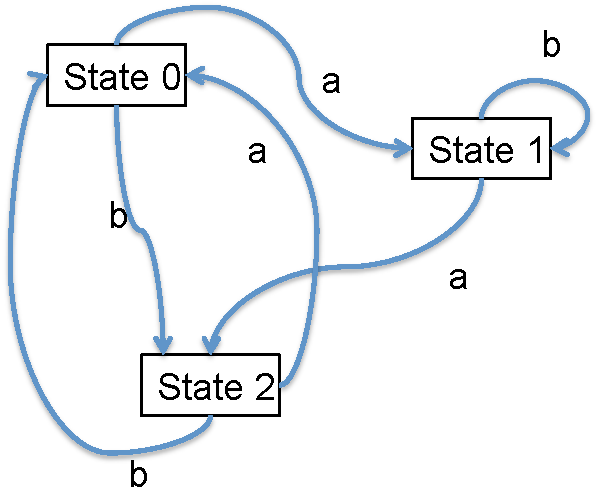
\includegraphics[height=.9in]{FSM1}}\hspace{.5in}
&\fbox{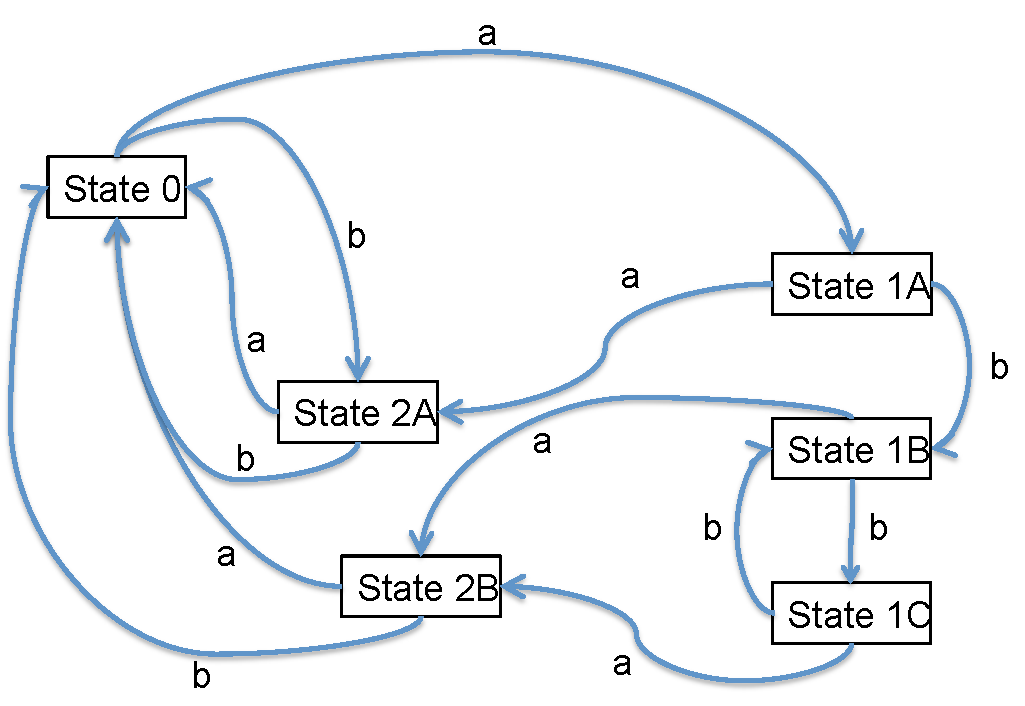
\includegraphics[height=1in]{FSM2}}\\\\
\tiny
\begin{tabular}{| l || l | l |}\bhline
\multicolumn{3}{|c|}{Original model $X\taking\mcM\to\Set$}\\\bhline
{\bf ID}&{\bf a}&{\bf b}\\\bbhline
State 0&State 1&State 2\\\hline
State 1& State 2& State 1\\\hline
State 2&State 0&State 0\\\bhline
\end{tabular}
\hspace{.5in}
&\tiny\begin{tabular}{| l || l | l |}\bhline
\multicolumn{3}{|c|}{Proposed model $Y\taking\mcM\to\Set$}\\\bhline
{\bf ID}&{\bf a}&{\bf b}\\\bbhline
State 0&State 1A&State 2A\\\hline
State 1A& State 2A& State 1B\\\hline
State 1B& State 2B& State 1C\\\hline
State 1C&State 2B&State 1B\\\hline
State 2A&State 0&State 0\\\hline
State 2B&State 0&State 0\\\bhline
\end{tabular}
\end{align*}

We can compose $X$ and $Y$ with $F$ as in the diagram below
$$
\xymatrix{\mcM'\ar[r]^F&\mcM\ar@/^1pc/[rr]^Y\ar@/_1pc/[rr]_X\ar@{}[rr]|{\alpha\Down}&&\Set}
$$
to get functors $Y\circ F$ and $X\circ F$, both of type $\mcM'\to\Set$. What would these be?
\footnote{The $p$-column comes from applying $b$ then $a$ then $a$, as specified above by $F$.}
\begin{center}\footnotesize
\begin{tabular}{| l || l | l | l |}\bhline
\multicolumn{4}{|c|}{$X\circ F$}\\\bhline
{\bf ID}&{\bf m}&{\bf n}&{\bf p}\\\bbhline
State 0&State 1&State 2&State 1\\\hline
State 1& State 2& State 1&State 0\\\hline
State 2&State 0&State 0&State 2\\\bhline
\end{tabular}
\hspace{.5in}
\begin{tabular}{| l || l | l | l |}\bhline
\multicolumn{4}{|c|}{$Y\circ F$}\\\bhline
{\bf ID}&{\bf m}&{\bf n}&{\bf p}\\\bbhline
State 0&State 1A&State 2A&State 1A\\\hline
State 1A& State 2A& State 1B&State 0\\\hline
State 1B& State 2B& State 1C&State 0\\\hline
State 1C&State 2B&State 1B&State 0\\\hline
State 2A&State 0&State 0&State 2A\\\hline
State 2B&State 0&State 0&State 2A\\\bhline
\end{tabular}
\end{center}

The map $\alpha$ is what sent both State 1A and State 1B in $Y$ to State 1 in $X$, and so on. We can see that “the same $\alpha$ works now:” the $p$ column of the table respects that mapping. But $\alpha$ was a natural transformation $Y\to X$ where as we need a natural transformation $Y\circ F\to X\circ F$. This is called {\em whiskering}. It is a kind of horizontal composition of natural transformation.

\end{example}

\begin{definition}[Whiskering]\index{natural transformation!whiskering of}\label{def:whiskering}

Let $\mcB,\mcC,\mcD,$ and $\mcE$ be categories, let $G_1,G_2\taking\mcC\to\mcD$ be functors, and let $\alpha\taking G_1\to G_2$ a natural transformation. Suppose that $F\taking\mcB\to\mcC$ (respectively $H\taking\mcD\to\mcE$) is a functor, depicted below:
$$
\xymatrix{\mcB\ar[r]^F&\mcC\ar@{}[r]|{\alpha\Down}\ar@/^1pc/[r]^{G_1}\ar@/_1pc/[r]_{G_2}&\mcD}
\hspace{.7in}
\left(\tn{respectively,}\hsp\xymatrix{\mcC\ar@{}[r]|{\alpha\Down}\ar@/^1pc/[r]^{G_1}\ar@/_1pc/[r]_{G_2}&\mcD\ar[r]^H&\mcE}\right),
$$
Then the {\em pre-whiskering of $\alpha$ by $F$}, denoted $\alpha\diamond F\taking G_1\circ F\to G_2\circ F$ (respectively, the {\em post-whiskering of $\alpha$ by $H$}, denoted $H\diamond\alpha\taking H\circ G_1\to H\circ G_2$) is defined as follows.\index{a symbol!$\diamond$}

For each $b\in\Ob(\mcB)$ the component $(\alpha\diamond F)_b\taking G_1\circ F(b)\to G_2\circ F(b)$ is defined to be $\alpha_{F(b)}$. (Respectively, for each $c\in\Ob(\mcC)$ the component $(H\diamond\alpha)_c\taking H\circ G_1(c)\to H\circ G_2(c)$ is defined to be $H(\alpha_c)$.) Checking that the naturality squares (in each case) is straightforward.

\end{definition}

The rest of this section can safely be skipped; I include it only for my own sense of completeness.

\begin{definition}[Horizontal composition of natural transformations]\index{natural transformation!horizontal composition of}\label{def:horizontal comp of nt}

Let $\mcB,\mcC,$ and $\mcD$ be categories, let $F_1,F_2\taking\mcB\to\mcC$ and $G_1,G_2\taking\mcC\to\mcD$ be functors, and let $\alpha\taking F_1\to F_2$ and $\beta\taking G_1\to G_2$ be natural transformations, as depicted below:
$$
\xymatrix{\mcB\ar@{}[r]|{\alpha\Down}\ar@/^1pc/[r]^{F_1}\ar@/_1pc/[r]_{F_2}&\mcC\ar@{}[r]|{\beta\Down}\ar@/^1pc/[r]^{G_1}\ar@/_1pc/[r]_{G_2}&\mcD}
$$
By pre- and post-whiskering in one order or the other we get the following diagram
$$
\xymatrix{
G_1\circ F_1\ar[r]^{G_1\diamond\alpha}\ar[d]_{\beta\diamond F_1}&G_1\circ F_2\ar[d]^{\beta\diamond F_2}\\
G_2\circ F_1\ar[r]_{G_2\diamond\alpha}&G_2\circ F_2}
$$
It is straightforward to show that this diagram commutes, so we can take the composition to be our definition of the horizontal composition 
$$\beta\diamond\alpha\taking G_1\circ F_1\to G_2\circ F_2.$$

\end{definition}

\begin{remark}

Whiskering a natural transformation $\alpha$ with a functor $F$ is the same thing as horizontally composing $\alpha$ with the identity natural transformation $\id_F$. This is true for both pre- and post- whiskering. For example in the notation of Definition \ref{def:whiskering} we have 
$$\alpha\diamond F = \alpha\diamond\id_F\hsp\tn{and}\hsp H\diamond\alpha=\id_H\diamond\alpha.$$

\end{remark}

\begin{remark}

All of the above is somehow similar to the world of paths inside a database schema $\mcS$, as seen in Definition \ref{def:congruence}. Indeed, a congruence on the paths of $\mcS$ is an equivalence relation that is closed under composition. The equivalence relation part is analogous to the fact that natural transformations can be composed vertically. The closure under composition part (Properties (3) and (4) in Definition \ref{def:congruence}) is analogous to pre- and post whiskering. See also Lemma \ref{lemma:composing PEDs}. 

This is being mentioned only as a curiosity and a way for the reader to draw connections, not with any additional purpose at this time.

\end{remark}

\begin{theorem}\index{natural transformation!interchange}
$$
\xymatrix{
&\ar@{}[d]|(.65){\alpha_1\Down}&&\ar@{}[d]|(.65){\beta_1\Down}\\
\mcC\ar@/^2pc/[rr]^{F_1}\ar[rr]|{F_2}\ar@/_2pc/[rr]_{F_3}&&\mcD\ar@/^2pc/[rr]^{G_1}\ar[rr]|{G_2}\ar@/_2pc/[rr]_{G_3}&&\mcE\\
&\ar@{}[u]|(.65){\alpha_2\Down}&&\ar@{}[u]|(.65){\beta_2\Down}}
$$
Given a setup of categories, functors, and natural transformations as above, we have
$$(\beta_2\circ\beta_1)\diamond(\alpha_2\circ\alpha_1)\;=\;(\beta_2\diamond\alpha_2)\circ(\beta_1\diamond\alpha_1).$$

\end{theorem}

\begin{proof}

One need only observe that each square in the following diagram commutes, so following the outer path $(\beta_2\circ\beta_1)\diamond(\alpha_2\circ\alpha_1)$ yields the same morphism as following the diagonal path $;(\beta_2\diamond\alpha_2)\circ(\beta_1\diamond\alpha_1)$:
$$
\xymatrix{
G_1F_1\ar[r]^{G_1\diamond\alpha_1}\ar[d]_{\beta_1\diamond F_1}&G_1F_2\ar[r]^{G_1\diamond\alpha_2}\ar[d]_{\beta_1\diamond F_2}&G_1F_3\ar[d]^{\beta_1\diamond F_3}\\
G_2F_1\ar[r]^{G_2\diamond\alpha_1}\ar[d]_{\beta_2\diamond F_1}&G_2F_2\ar[r]^{G_2\diamond\alpha_2}\ar[d]_{\beta_2\diamond F_2}&G_2F_3\ar[d]^{\beta_2\diamond F_3}\\
G_3F_1\ar[r]_{G_3\diamond\alpha_1}&G_3F_2\ar[r]_{G_3\diamond\alpha_2}&G_3F_3
}
$$


\end{proof}

%%%% Subsection %%%%

\subsection{\caseENGRUS{The category of instances on a database schema}{ / }{Категория экземпляров схемы базы данных}}\index{a category!$\mcC\set$}\index{database!category of instances on}

In Section \ref{sec:schemas and cats intro} we showed that schemas are presentations of categories, and we will show in Section \ref{sec:cat equiv sch} that in fact the category of schemas is equivalent to the category of categories. In this section we therefore take license to blur the distinction between schemas and categories.

If $\mcC$ is a schema, i.e. a category, then as we discussed in Section \ref{sec:instances}, an instance on $\mcC$ is a functor $I\taking\mcC\to\Set$. But now we have a notion beyond categories and functors, namely that of natural transformations. So we make the following definition.

\begin{definition}\label{def:mcC-set}

Let $\mcC$ be a schema (or category). The {\em category of instances on $\mcC$}, denoted $\mcC\set$, is $\Fun(\mcC,\Set)$. Its objects are $\mcC$-instances (i.e. functors $\mcC\to\Set)$ and its morphisms are natural transformations.

\end{definition}

\begin{remark}

One might object to Definition \ref{def:mcC-set} on the grounds that database instances should not be infinite. This is a reasonable perspective, so it is a pleasant fact that the above definition can be modified easily to accomodate it. The subcategory $\Fin$ (see Example \ref{ex:Fin}) of finite sets can be substituted for $\Set$ in Definition \ref{def:mcC-set}. One could define the {\em category of finite instances on $\mcC$} as $\mcC-\Fin=\Fun(\mcC,\Fin)$. Almost all of the ideas in this book will make perfect sense in $\mcC-\Fin$.

\end{remark}

Natural transformations should serve as some kind of morphism between instances on the same schema. How are we to interpret a natural transformation $\alpha\taking I\to J$ between database instances $I,J\taking\mcC\to\Set$? 

Our first clue comes from Application \ref{app:change of fsm}. There we considered the case of a monoid $\mcM$, and we thought about a natural transformation between two functors $X,Y\taking\mcM\to\Set$, considered as different finite state machines. The notion of natural transformation captured the idea of one model being a refinement of another. This same kind of idea works for databases with more than one table (categories with more than one object), but the whole thing is a bit opaque. Let's work it through slowly.

\begin{example}\label{ex:nts on term}
Let us consider the terminal schema, $\ul{1}\iso\fbox{$\bullet^{\tn{Grapes}}$}$. An instance is a functor $\ul{1}\to\Set$ and it is easy to see that this is the same thing as just a set. A natural transformation $\alpha\taking I\to J$ is a function from set $I$ to set $J$. In the standard table view, we might have $I$ and $J$ as below:
\begin{center}
\begin{tabular}{| l ||}\bhline
\multicolumn{1}{| c |}{Grapes $(I)$}\\\bhline
{\bf ID}\\\bbhline
Grape 1\\\hline
Grape 3\\\hline
Grape 4\\\bhline
\end{tabular}
\hspace{1in}
\begin{tabular}{| l ||}\bhline
\multicolumn{1}{| c |}{Grapes $(J)$}\\\bhline
{\bf ID}\\\bbhline
Jan1-01\\\hline
Jan1-02\\\hline
Jan1-03\\\hline
Jan1-04\\\hline
Jan3-01\\\hline
Jan4-01\\\hline
Jan4-02\\\bhline
\end{tabular}
\end{center}

There are 343 natural transformations $I\to J$. Perhaps some of them make more sense than others; e.g. we could hope that the numbers in $I$ corresponded to the numbers after the dash in $J$, or perhaps to what seems to be the date in January. But it could be that the rows in $J$ correspond to batches, and all three grapes in $I$ are part of the first batch on Jan-1. The notion of natural transformation is a mathematical one.
\end{example}

\begin{exercise}\label{exc:indexed sets as functors}\index{indexed set!as functor}
Recall the notion of set-indexed sets from Definition \ref{def:indexed sets}. Let $A$ be a set, and come up with a schema $\mcA$ such that instances on $\mcA$ are $A$-indexed sets. Is our current notion of morphism between instances (i.e. natural transformations) well-aligned with the above definition of “mapping of $A$-indexed sets”?
\end{exercise}

For a general schema (or category) $\mcC$, let us think through what a morphism $\alpha\taking I\to J$ between instances $I,J\taking\mcC\to\Set$ is. For each object $c\in\Ob(\mcC)$ there is a component $\alpha_c\taking I(c)\to J(c)$. This means that just like in Example \ref{ex:nts on term}, there is for each table $c$ a function from the rows in $I$'s manifestation of $c$ to the rows in $J$'s manifestation of $c$. So to make a natural transformation, such a function has to be specified table by table. But then we have to contend with naturality squares, one for every arrow in $\mcC$. Arrows in $\mcC$ correspond to foreign key columns in the database. The naturality requirement was already covered in Application \ref{app:change of fsm} (and see especially how (\ref{dia:naturality squares for fsm}) is checked in (\ref{dia:naturality for a}) and (\ref{dia:naturality for b})).

\begin{example}\label{ex:graph hom as NT done out}\index{graph homomorphism!as functor}

We saw in Section \ref{sec:graphs as functors} that graphs can be regarded as functors $\mcG\to\Set$, where $\mcG\iso\GrIn$ is the “schema for graphs” shown here: 
$$\mcG:=\fbox{\xymatrix{\LTO{Arrow}\ar@<.5ex>[r]^{src}\ar@<-.5ex>[r]_{tgt}&\LTO{Vertex}}}$$\index{a schema!indexing graphs}


A database instance $I\taking\mcG\to\Set$ on $\mcG$ consists of two tables. Here is an example instance:
\begin{align*}
I:=\parbox{2in}{\fbox{\xymatrix{\bullet^v\ar[r]^f&\bullet^w\ar@/_1pc/[r]_h\ar@/^1pc/[r]^g&\bullet^x}}}
\hspace{.5in}
\begin{array}{| l || l | l |}\bhline
\multicolumn{3}{|c|}{{\tt Arrow}\;\; (I)}\\\bhline
{\bf ID}&{\bf src}&{\bf tgt}\\\bbhline
f&v&w\\\hline
g&w&x\\\hline
h&w&x\\\bhline
\end{array}
\hspace{.5in}
\begin{array}{| l ||}\bhline
\multicolumn{1}{|c|}{{\tt Vertex}\;\; (I)}\\\bhline
{\bf ID}\\\bbhline
v\\\hline
w\\\hline
x\\\bhline
\end{array}
\end{align*}
To discuss natural transformations, we need two instances. Here is another, $J\taking\mcG\to\Set$,
\begin{align*}
J:=\parbox{2in}{\fbox{\xymatrix{
\LMO{q}\ar[r]^i&\LMO{r}\ar@/^1pc/[r]^j&\LMO{s}\ar@/^1pc/[l]^k\ar[r]^\ell&\LMO{t}\\&&&\LMO{u}}}}
\hspace{.5in}
\begin{array}{| l || l | l |}\bhline
\multicolumn{3}{|c|}{{\tt Arrow}\;\; (J)}\\\bhline
{\bf ID}&{\bf src}&{\bf tgt}\\\bbhline
i&q&r\\\hline
j&r&s\\\hline
k&s&r\\\hline
\ell&s&t\\\bhline
\end{array}
\hspace{.5in}
\begin{array}{| l ||}\bhline
\multicolumn{1}{|c|}{{\tt Vertex}\;\; (J)}\\\bhline
{\bf ID}\\\bbhline
q\\\hline
r\\\hline
s\\\hline
t\\\hline
u\\\bhline
\end{array}
\end{align*}
To give a natural transformation $\alpha\taking I\to J$, we give two components: one for arrows and one for vertices. We need to say where each vertex in $I$ goes in $J$ and we need to say where each arrow in $I$ goes in $J$. The naturality squares insist that if we specify that $g\mapsto j$, for example, then we better specify that$w\mapsto r$ and that $x\mapsto s$. What a computer is very good at, but a human is fairly slow at, is checking that a given pair of components (arrows and vertices) really is natural. 

There are 8000 ways to come up with component functions $\alpha_{{\tt Arrow}}$ and $\alpha_{{\tt Vertex}}$, but precisely four natural transformations, i.e. four graph homomorphisms, $I\to J$; the other 7996 are haphazard flingings of arrows to arrows and vertices to vertices without any regard to sources and targets. We briefly describe the four now. 

First off, nothing can be sent to $u$ because arrows must go to arrows and $u$ touches no arrows. If we send $v\mapsto q$ then $f$ must map to $i$, and $w$ must map to $r$, and both $g$ and $h$ must map to $j$, and $x$ must map to $s$. If we send $v\mapsto r$ then there are two choices for $g$ and $h$. If we send $v\mapsto s$ then there's one way to obtain a graph morphism. If we try to send $v\mapsto^?t$, we fail. All of this can be seen by staring at the tables rather than at the pictorial representations of the graphs; the human eye understands these pictures better, but the computer understands the tables better.

\end{example}

\begin{exercise}
If $I,J\taking\mcG\to\Set$ are as in Example \ref{ex:graph hom as NT done out}, how many natural transformations are there $J\to I$?
\end{exercise}

\begin{exercise}
Let $Y_A\taking\mcG\to\Set$ denote the instance below:
\begin{align*}
\begin{array}{| l || l | l |}\bhline
\multicolumn{3}{|c|}{{\tt Arrow}\;\; (Y_A)}\\\bhline
{\bf ID}&{\bf src}&{\bf tgt}\\\bbhline
a&v_0&v_1\\\bhline
\end{array}
\hspace{.5in}
\begin{array}{| l ||}\bhline
\multicolumn{1}{|c|}{{\tt Vertex}\;\; (Y_A)}\\\bhline
{\bf ID}\\\bbhline
v_0\\\hline
v_1\\\bhline
\end{array}
\end{align*}
Let $I\taking\mcG\to\Set$ be as in Example \ref{ex:graph hom as NT done out}.
\sexc How many natural transformations are there $Y_A\to I$?
\item With $J$ as above, how many natural transformations are there $Y_A\to J$?
\item Do you have any conjecture about the way natural transformations $Y_A\to X$ behave for arbitrary graphs $X\taking\mcG\to\Set$?
\endsexc
\end{exercise}

In terms of databases, this notion of instance morphism $I\to J$ is fairly benign. For every table its a mapping from the set of rows in $I$'s version of the table to $J$'s version of the table, such that all the foreign keys are respected. We will see that this notion of morphism has excellent formal properties, so that projections, unions, and joins of tables (the typical database operations) would be predicted to be “obviously interesting” by a category theorist who had no idea what a database was.
\footnote{More precisely, given a functor between schemas $F\taking\mcC\to\mcD$, the pullback $\Delta_F\taking\mcD\set\to\mcC\set$, its left $\Sigma_F$ and its right adjoint $\Pi_F$ constitute these important queries. See Section \ref{sec:data migration}.}

However, something is also missing from the natural transformation picture. A very important occurrence in the world of databases is the update. Everyone can understand this: a person makes a change in one of the tables, like changing your address from Cambridge, MA to Hereford, UK. Most such arbitrary changes of database instance are not “natural”, in that the new linking pattern is incompatible with the old.

It is interesting to consider how updates of $\mcC$-instances should be understood category theoretically. We might want a category $Upd_\mcC$ whose objects are $\mcC$-instances and whose morphisms are updates. But then what is the composition formula? Is there a unique morphism $I\to J$ whenever $J$ can be obtained as an update on $I$? Because in that case, we would be defining $Upd_\mcC$ to be the indiscrete category on the set of $\mcC$-instances (see Example \ref{ex:indiscrete cat equiv to terminal}).

\begin{exercise}
Research project: Can you come up with a satisfactory way to model database updates category-theoretically? Let $\NN$ be the category
$$[\NN]:=\xymatrix{\LMO{0}\ar[r]&\LMO{1}\ar[r]&\LMO{2}\ar[r]&\cdots}$$ 
representing a discrete timeline. A place to start might be to use something like the slice category $\Cat_{/[\NN]}$ where the fiber over each object in $\NN$ is a snapshot of the database in time. Can you make this work?
\end{exercise}


%%%% Subsection %%%%

\subsection{\caseENGRUS{Equivalence of categories}{ / }{Эквивалентность категорий}}\label{sec:equivalence of cats}

We have a category $\Cat$ of categories, and in every category there is a notion of isomorphism between objects: one morphism each way, such that each round-trip composition is the identity. An isomorphism in $\Cat$, therefore, takes place between two categories, say $\mcC$ and $\mcD$: it is a functor $F\taking\mcC\to\mcD$ and a functor $G\taking\mcD\to\mcC$ such that $G\circ F=\id_\mcC$ and $F\circ G=\id_\mcD$. 

It turns out that categories are often similar enough to be considered equivalent without being isomorphic. For this reason, the notion of isomorphism is considered “too strong” to be useful for categories. The feeling to a category theorist might be akin to saying that two material samples are the same if there is an atom-by-atom matching, or that two words are the same if they are written in the same font, of the same size, by the same person, in the same state of mind. 

As reasonable as isomorphism is as a notion {\em in} most categories, it fails to be the “right notion” {\em about} categories. The reason is that {\em in} categories there are objects and morphisms, whereas when we talk {\em about} categories, we have categories and functors, plus natural transformations. These serve as mappings between mappings, and this is not part of the structure of an ordinary category. In cases where a category $\mcC$ does have such mappings between mappings, it is often a “better notion” if we take that extra structure into account, like we will for categories. This whole subject leads us to the study of 2-categories (or $n$-categories, or $\infty$-categories), which we do not discuss in this book. See, for example, \cite{Le1} for an introduction.

Regardless, our purpose now is to explain this “good notion” of sameness for categories, namely {\em equivalences of categories}, which appropriately take natural transformations into account. Instead of “functors going both ways with round trips equal to identity”, which is required in order to be an isomorphism of categories, equivalence of categories demands “functors going both ways with round trips {\em isomorphic} to identity”.

\begin{definition}[Equivalence of categories]\label{def:equiv of cats}\index{category!equivalence of}

Let $\mcC$ and $\mcC'$ be categories. A functor $F\taking\mcC\to\mcC'$ is called {\em an equivalence of categories}, and denoted $F\taking\mcC\To{\simeq}\mcC'$,\index{a symbol!$\simeq$}
\footnote{The notation $\simeq$ has already been used for equivalences of paths in a schema. We do not mean to equate these ideas; we are just reusing the symbol. Hopefully no confusion will arise.}
 if there exists a functor $F'\taking\mcC'\to\mcC$ and natural isomorphisms $\alpha\taking \id_\mcC\To{\iso}F'\circ F$ and $\alpha'\taking\id_{\mcC'}\To{\iso}F\circ F'$. In this case we say that $F$ and $F'$ are {\em mutually inverse equivalences}.

\end{definition}

Unpacking a bit, suppose we are given functors $F\taking\mcC\to\mcC'$ and $F'\taking\mcC'\to\mcC$. We want to know something about the roundtrips on $\mcC$ and on $\mcC'$; we want to know the same kind of information about each roundtrip, so let's concentrate on the $\mcC$ side. We want to know something about $F'\circ F\taking\mcC\to\mcC$, so let's name it $i\taking\mcC\to\mcC$; we want to know that $i$ is a natural isomorphism. That is, for every $c\in\Ob(\mcC)$ we want an isomorphism $\alpha_c\taking c\To{\iso} i(c)$, and we want to know that these isomorphisms are picked carefully enough that given $g\taking c\to c'$ in $\mcC$, the choice of isomorphisms for $c$ and $c'$ are compatible,
$$\xymatrix{c\ar[r]^{\alpha_c}\ar[d]_g&i(c)\ar[d]^{i(g)}\\c'\ar[r]_{\alpha_{c'}}&i(c').}$$
To be an equivalence, the same has to hold for the other roundtrip, $i'=F\circ F'\taking\mcC'\to\mcC'.$

\begin{exercise}
Let $\mcC$ and $\mcC'$ be categories. Suppose that $F\taking\mcC\to\mcC'$ is an isomorphism of categories.
\sexc Is it an equivalence of categories?
\item What are the components of $\alpha$ and $\alpha'$ (with notation as in Definition \ref{def:equiv of cats})?
\endsexc
\end{exercise}

\begin{example}\label{ex:indiscrete cat equiv to terminal}

Let $S$ be a set and let $S\times S\ss S\times S$ be the complete relation on $S$, which is a preorder $K_S$. Recall from Proposition \ref{prop:preorders to cats} that we have a functor $i\taking\PrO\to\Cat$,\index{a functor!$\PrO\to\Cat$} and the resulting category $i(K_S)$ is called the {\em indiscrete category on $S$}; it has objects $S$ and a single morphism between every pair of objects. Here is a picture of $K_{\{1,2,3\}}$:
$$\xymatrix@=15pt{\LMO{1}\ar@(l,u)[]\ar@/^.5pc/[rr]\ar@/^.5pc/[rdd]&&\LMO{2}\ar@(u,r)[]\ar@/^.5pc/[ll]\ar@/^.5pc/[ldd]\\\\&\LMO{3}\ar@(dr,dl)[]_~\ar@/^.5pc/[uur]\ar@/^.5pc/[uul]}$$

It is easy check that $K_{\ul{1}}$, the indiscrete category on one element, is isomorphic to $\ul{1}$, the discrete category on one object, also known as the terminal category (see Exercise \ref{exc:term cat}). The category $\ul{1}$ consists of one object, its identity morphism, and nothing else. 

The only way that $K_S$ can be isomorphic to $\ul{1}$ is if $S$ has one element.
\footnote{One way to see this is that by Exercise \ref{exc:Ob is a functor}, we have a functor $\Ob\taking\Cat\to\Set$, and we know by Exercise \ref{exc:functors preserve isos} that functors preserve isomorphisms, so an isomorphism between categories must restrict to an isomorphism between their sets of objects. The only sets that are isomorphic to $\ul{1}$ have one element.} 
On the other hand, there is an equivalence of categories $$K_S\simeq\ul{1}$$ for every set $S\neq\emptyset$. 

In fact, there are many such equivalences, one for each element of $S$. To see this, let $S$ be a nonempty set and choose an element $s_0\in S$. For every $s\in S$, there is a unique isomorphism $k_s\taking s\To{\iso}s_0$ in $K_S$. Let $F\taking K_S\to\ul{1}$ be the only possible functor (see Exercise \ref{exc:term cat}), and let $F'\taking\ul{1}\to K_S$ send the unique object in $\ul{1}$ to the object $s_0$. 

Note that $F'\circ F=\id_{\ul{1}}\taking\ul{1}\to\ul{1}$ is the identity, but that $F\circ F'\taking K_S\to K_S$ sends everything to $s_0$. Let $\alpha=\id_{\ul{1}}$ and define $\alpha'\taking\id_{K_S}\to F\circ F'$ by $\alpha'_s=k_s$. Note that $\alpha'_s$ is an isomorphism for each $s\in\Ob(K_S)$, and note that $\alpha'$ is a natural transformation (hence natural isomorphism) because every possible square commutes in $K_S$. This completes the proof, initiated in the paragraph above, that the category $K_S$ is equivalent to $\ul{1}$ for every nonempty set $S$, and that this fact can be witnessed by any element $s_0\in S$.

\end{example}

\begin{example}\label{ex:finite linear orders}

Consider the category $\FLin$, described in Example \ref{ex:FLin}, of finite nonempty linear orders. For every natural number $n\in\NN$, let $[n]\in\Ob(\FLin)$ denote the linear order shown in Example \ref{ex:finite lo}. Define a category $\bD$\index{a category!$\bD$} whose objects are given by $\Ob(\bD)=\{[n]\|n\in\NN\}$ and with $\Hom_{\bD}([m],[n])=\Hom_{\FLin}([m],[n])$. The difference between $\FLin$ and $\bD$ is only that objects in $\FLin$ may have “funny labels”, e.g. 
$$\xymatrix{\LMO{5}\ar[r]&\LMO{x}\ar[r]&\LMO{“Sam”}}$$ 
whereas objects in $\bD$ all have standard labels, e.g.
$$\xymatrix{\LMO{0}\ar[r]&\LMO{1}\ar[r]&\LMO{2}}$$
Clearly $\FLin$ is a much larger category, and yet feels like it is “pretty much the same as” $\bD$. Justly, they are equivalent, $\FLin\simeq\bD$. 

The functor $F'\taking\bD\to\FLin$\index{a functor!$\bD\to\FLin$} is the inclusion; the functor $F\taking\FLin\to\bD$ sends every finite nonempty linear order $X\in\Ob(\FLin)$ to the object $F(X):=[n]\in\bD$, where $\Ob(X)\iso\{0,1,\ldots,n\}$. For each such $X$ there is a unique isomorphism $\alpha_X\taking X\To{\iso}[n]$, and these fit together into
\footnote{The phrase “these fit together into” is suggestive shorthand for, and thus can be replaced with, the phrase “the naturality squares commute for these components, so together they constitute”.}
the required natural isomorphism $\id_{\FLin}\to F'\circ F$. The other natural isomorphism $\alpha'\taking\id_{\bD}\to F\circ F'$ is the identity.

\end{example}

\begin{exercise}
Recall from Definition \ref{def:cardinality} that a set $X$ is called finite if there exists a natural number $n\in\NN$ and an isomorphism of sets $X\to\ul{n}$. Let $\Fin$\index{a category!$\Fin$} denote the category whose objects are the finite sets and whose morphisms are the functions. Let $\mcS$ denote the category whose objects are the sets $\ul{n}$ and whose morphisms are again the functions. For every object $X\in\Ob(\Fin)$ there exists an isomorphism $p_X\taking X\to\ul{n}$ for some unique object $\ul{n}\in\Ob(\mcS)$. Find an equivalence of categories $\Fin\To{\simeq}\mcS$. 
\end{exercise}

\begin{exercise}
We say that two categories $\mcC$ and $\mcD$ are equivalent if there exists an equivalence of categories between them. Show that the relation of “being equivalent” is an equivalence relation on $\Ob(\Cat)$.
\end{exercise}

\begin{example}\label{ex:Z1 not equiv Z2}

Consider the group $\ZZ_2:=(\{0,1\},0,+)$, where $1+1=0$. As a category, $\ZZ_2$ has one object $\monOb$ and two morphisms, namely $0,1$, such that $0$ is the identity. Since $\ZZ_2$ is a group, the morphism $1\taking\monOb\to\monOb$ must have an inverse $x$, meaning $1+x=0$, and $x=1$ is the only solution.

The point is that the morphism $1$ in $\ZZ_2$ is an isomorphism. Let $\mcC=\ul{1}$ be the terminal category as in Exercise \ref{exc:term cat}. One might accidentally believe that $\mcC$ is equivalent to $\ZZ_2$, but this is not the case! The argument in favor of the accidental belief is that we have unique functors $F\taking\ZZ_2\to\mcC$ and $F'\taking\mcC\to\ZZ_2$ (and this is true); the roundtrip $F\circ F'\taking\mcC\to\mcC$ is the identity (and this is true); and for the roundtrip $F'\circ F\taking\ZZ_2\to\ZZ_2$ both morphisms in $\ZZ_2$ are isomorphisms, so any choice of morphism $\alpha_\monOb\taking\monOb\to F'\circ F(\monOb)$ will be an isomorphism (and this is true). The problem is that no such $\alpha_\monOb$ will be a natural transformation.

When we roundtrip $F'\circ F\taking\ZZ_2\to\ZZ_2$, the image of $1\taking\monOb\to\monOb$ is $F'\circ F(1)=0=\id_{\monOb}$. So the naturality square for the morphism $1$ looks like this:
$$
\xymatrix{\monOb\ar[r]^{\alpha_\monOb}\ar[d]_{1}&\monOb\ar[d]^{0=F'\circ F(1)}\\\monOb\ar[r]_{\alpha_\monOb}&\monOb}
$$
where we still haven't decided whether we want $\alpha_\monOb$ to be $0$ or $1$. Unfortunately, neither choice works (i.e. for neither choice will the diagram commute) because $x+1\neq x+0$ in $\ZZ_2$.

\end{example}

\begin{definition}[Skeleton]\index{skeleton}

Let $\mcC$ be a category. We saw in Lemma \ref{lemma:isomorphic ER} that the relation of “being isomorphic” is an equivalence relation $\cong$ on $\Ob(\mcC)$. An {\em election in $\mcC$} is a choice $E$ of the following sort:
\begin{itemize}
\item for each $\cong$-equivalence class $S\ss\Ob(\mcC)$ a choice of object $s_E\in S$, called the {\em elected object for $S$}, and
\item for each object $c\in\Ob(\mcC)$ a choice of isomorphism $i_c\taking s_E\to c$ and $j_c\taking c\to s_E$ with $i_c\circ j_c=\id_c$ and $j_c\circ i_c=\id_{s_E}$, where $s_E$ is an elected object (depending on $c$).
\end{itemize}
Given an election $E$ in $\mcC$, there is a category called the {\em $E$-elected skeleton of $\mcC$}, denoted $\Skel_E(\mcC)$, whose objects are the elected objects and whose morphisms $s\to t$ for any elected objects $s,t\in\Ob(\mcC)$ are given by $\Hom_{\Skel_E(\mcC)}(s,t)=\Hom_\mcC(s,t)$. Any object $c\in\Ob(\mcC)$ is isomorphic to a unique elected object $s_E$; we refer to $s_E$ as the {\em elected representative} of $c$; we refer to the isomorphisms $i_c$ and $j_c$ as the {\em representing isomorphisms} for $c$.

\end{definition}

\begin{proposition}

Let $\mcC$ be a category and let $E$ be an election in $\mcC$. There is an equivalence of categories $$\Skel_E(\mcC)\simeq\mcC.$$

\end{proposition}

\begin{proof}

The functor $F'\taking\Skel_E(\mcC)\to\mcC$ is the inclusion. The functor $F\taking\mcC\to\Skel_E(\mcC)$ sends each object in $\mcC$ to its elected representative. Given objects $c,c'\in\Ob(\mcC)$ with elected representatives $s,t$ respectively, and given a morphism $g\taking c\to c'$ in $\mcC$, let $i_c,j_c,i_{c'},$ and $j_{c'}$ be the representing isomorphisms, and define $F(g)\taking s\to t$ to be the composite 
$$\xymatrix{s\ar[r]^{i_c}&c\ar[r]^g&c'\ar[r]^{j_{c'}}&t.}$$
This is functorial because it sends the identity to the identity and $F(g\circ g')=F(g)\circ F(g')$.

The composite $F\circ F'\taking\Skel_E(\mcC)\to\Skel_E(\mcC)$ is the identity. For each $c\in\Ob(\mcC)$ define $\alpha_c\taking c\To{\iso} F'\circ F(c)$ by  $\alpha_c:=j_c$. Given $g\taking c\to c'$ the required naturality square is shown to the left below:
$$
\xymatrix@=40pt{
c\ar[r]^{j_c}\ar[d]_{g}\ar@{}[dr]|{?}&s\ar[r]^{i_c}\ar[d]^{F'\circ F(g)}&c\ar[d]^g\\
c'\ar[r]_{j_c'}&t&c'\ar[l]^{j_c'}}
$$
The right-hand part commutes by definition of $F$ and $F'$; i.e. $j'\circ g\circ i_c=F'\circ F(g)$. The left-hand square commutes because $i_c\circ j_c=\id_c$.

\end{proof}

\begin{definition}

A {\em skeleton of $\mcC$} is a category $\mcS$, equivalent to $\mcC$, such that for any two objects $s,s'\in\Ob(\mcS)$, if $s\iso s'$ then $s=s'$. 

\end{definition}

\begin{exercise}
Let $\mcP$ be a preorder (considered as a category).
\sexc If $\mcP'$ is a skeleton of $\mcP$, is it a partial order?
\item Is every partial order the skeleton of some preorder?
\endsexc
\end{exercise}

\begin{definition}[Full and faithful functors]\label{def:full faithful}\index{functor!full}\index{functor!faithful}

Let $\mcC$ and $\mcD$ be categories, and let $F\taking\mcC\to\mcD$ be a functor. For any two objects $c,c'\in\Ob(\mcC)$, we have a function $\Hom_F(c,c')\taking\Hom_\mcC(c,c')\to\Hom_\mcD(F(c),F(c'))$ guaranteed by the definition of functor.
We say that $F$ is {\em a full functor} if $\Hom_F(c,c')$ is surjective for every $c,c'$.
We say that $F$ is {\em a faithful functor} if $\Hom_F(c,c')$ is injective for every $c,c'$. We say that $F$ is {\em a fully faithful functor} if $\Hom_F(c,c')$ is bijective for every $c,c'$.

\end{definition}

\begin{exercise}
Let $\ul{1}$ and $\ul{2}$ be the discrete categories on one and two objects, respectively. There is only one functor $\ul{2}\to\ul{1}$.
\sexc Is it full?
\item Is it faithful?
\endsexc
\end{exercise}

\begin{exercise}\label{exc:empty fully faithful}
Let $\ul{0}$ denote the empty category, and let $\mcC$ be any category. There is a unique functor $F\taking \ul{0}\to\mcC$.
\sexc For general $\mcC$ will $F$ be full?
\item For general $\mcC$ will $F$ be faithful?
\item For general $\mcC$ will $F$ be an equivalence of categories?
\endsexc
\end{exercise}

\begin{proposition}

Let $\mcC$ and $\mcC'$ be categories and let $F\taking\mcC\to\mcC'$ be an equivalence of categories. Then $F$ is fully faithful.

\end{proposition}

\begin{proof}

Suppose $F$ is an equivalence, so we can find a functor $F'\taking\mcC'\to\mcC$ and natural isomorphisms $\alpha\taking\id_\mcC\To{\iso}F'\circ F$ and $\alpha'\taking\id_{\mcC'}\To{\iso} F\circ F'$. We need to know that for any objects $c,d\in\Ob(\mcC)$, the map $$\Hom_F(c,d)\taking\Hom_\mcC(c,d)\to\Hom_{\mcC'}(Fc,Fd)$$ is bijective. Consider the following diagram 
$$
\xymatrix{
\Hom_\mcC(c,d)\ar[rr]^{\Hom_F(c,d)}\ar[ddrr]_\alpha&&\Hom_{\mcC'}(Fc,Fd)\ar[ddrr]^{\alpha'}\ar[dd]^{\Hom_{F'}(Fc,Fd)}\\\\
&&\Hom_\mcC(F'Fc,F'Fd)\ar[rr]_{\Hom_{F}(F'Fc,F'Fd)}&&\Hom_{\mcC'}(FF'Fc,FF'Fd)
}
$$
The fact that $\alpha$ is bijective implies that the vertical function is surjective. The fact that $\alpha'$ is bijective implies that the vertical function is injective, so it is bijective. This implies that $\Hom_F(c,d)$ is bijective as well.

\end{proof}

\begin{exercise}
Let $\ZZ_2$ be the group (as category) from Example \ref{ex:Z1 not equiv Z2}. Are there any fully faithful functors $\ZZ_2\to\ul{1}$?
\end{exercise}

